\chapter{ANALISIS DAN PERANCANGAN SISTEM} \label{chapter:analisis dan perancangan sistem}
\tab Pada bab ini akan dijelaskan mengenai analisis dan perancangan sistem perangkat lunak yang akan dibangun, meliputi struktur data, algoritme, dan arsitektur aplikasi. 

\section{Daftar Notasi}
\tab Tabel \ref{tab:daftar-notasi-2} menunjukkan daftar notasi yang digunakan dalam bab ini beserta deskripsinya.

\begin{longtable}{| p{3cm} | p{7cm} |} 
	\caption{Daftar Notasi (2) \label{tab:daftar-notasi-2}}\\
	\hline
	\multicolumn{1}{|p{3cm}|}{\textbf{Notasi}} & \multicolumn{1}{|p{7cm}|}{\textbf{Deskripsi}}\\ \hline
	\hline
	\endfirsthead
	\hline
	\multicolumn{1}{|p{3cm}|}{\textbf{Notasi}} & \multicolumn{1}{|p{7cm}|}{\textbf{Deskripsi}}\\ \hline 
	\endhead
	$P$ & \textit{Dataset} produk\\ \hline
	$C$ & \textit{Dataset} pelanggan (preferensi pelanggan)\\ \hline
	$D$ & $P \cup C$ \\ \hline
	$ob$ & Sebuah objek data pada $D$\\ \hline
	$ob_1 \prec ob_2$ & Objek data $ob_1$ mendominasi $ob_2$\\ \hline
	$ob_1 \prec_{ob_3} ob_2$ & Objek data $ob_1$ mendominasi $ob_2$ berdasarkan $ob_3$\\ \hline
	$p$ & Sebuah produk dalam $P$, $p \in P$\\ \hline
	$c$ & Seorang pelanggan dalam $C$, $c \in C$\\ \hline
	$d$ & Jumlah dimensi pada $D$\\ \hline
	$i$ & Dimensi ke-1, ..., $d$\\ \hline
	$j$ & Timestamp ke-1, 2, ..., dst\\ \hline
	$O$ & \textit{Orthant} atau daerah pada komputasi \textit{reverse skyline}\\ \hline
	$m$ & \textit{Midpoint} antar produk pada komputasi \textit{reverse skyline}\\ \hline
	$DSL(c)$ & Hasil \textit{dynamic skyline} dari pelanggan $c$\\ \hline
	$RSL(p)$ & Hasil \textit{reverse skyline} dari produk $p$\\ \hline
	$Pr(c, p|P)$ & Probabilitas produk $p$ dibeli oleh pelanggan $c$ \\ \hline
	$E(C, p|P)$ & Kontribusi pasar $p$\\ \hline
	$E(C, P'|P)$ & Kontribusi pasar subset $P'$ dari $P$ \\ \hline
	$k-MPP$ & \textit{k-Most Promising Products} \\ \hline
	$k-MPPTI$ & \textit{k-Most Promising Products in Time Intervals} \\ \hline
\end{longtable}

\section{Analisis Sistem}
\tab Analisis sistem dijelaskan dalam empat bagian, yakni analisis permasalahan, deskripsi umum sistem, fungsi sistem, dan analisis kebutuhan fungsional.

\subsection{Analisis Permasalahan}
\tab Permalasahan yang ingin diselesaikan pada Tugas Akhir ini adalah bagaimana menjawab kueri \textit{$k$-Most Promising Products} berbasis interval waktu ($k$-MPPTI). Interval waktu, dinotasikan dengan $[t_i:t_e ](t_i \leq t_e)$, digunakan untuk menentukan rentang waktu pencarian. Sehingga, kueri $k$-MPP yang sudah ada \cite{kmpp} dimodifikasi menjadi:
\begin{equation}\label{eq:kmppts}
k-MPPTI(P, C, k, [t_i:t_e])
\end{equation} 

Permasalahan ini tidak dapat langsung diselesaikan menggunakan metode dan algoritme yang sudah ada \cite{kmpp}. Sehingga, diperlukan pendekatan lain yang akan dijelaskan pada bagian perancangan sistem.

\subsection{Deskripsi Umum Sistem}
\tab Secara umum, sistem yang akan dibangun adalah sebuah sistem berbasis web yang dapat membantu pengguna untuk memilih \textit{k}-produk yang paling menjanjikan. Dikatakan "menjanjikan" jika produk tersebut memiliki kontribusi pasar yang besar.

Sistem ini memiliki dua proses utama, yaitu (1) \textit{data precomputing} untuk menghitung kontribusi pasar masing-masing produk dan (2) proses utama (selanjutnya akan disebut dengan \textit{query processing}) untuk memproses dan menampilkan hasil kueri pencarian yang dimasukkan oleh pengguna.

Sistem ini dibangun menggunakan arsitektur \textit{client}-\textit{server}. Aplikasi \textit{client} didesain berbasis web dengan memanfaatkan Flask \textit{microframework}, HTML, CSS, dan JavaScript. Selain itu, Flask juga digunakan sebagai \textit{webserver}. 

\subsection{Fungsi Sistem}
\tab Sistem yang akan dibangun memiliki beberapa fungsi utama sebagai berikut:
\begin{enumerate}
	\item Dapat menerima \textit{input} data berupa file dari pengguna
	\item Dapat menampilkan informasi dan pratinjau data yang di-\textit{input}-kan oleh pengguna
	\item Dapat menampilkan visualisasi data
	\item Dapat melakukan proses \textit{data pre-computing} menggunakan algoritme yang dipilih oleh pengguna
	\item Dapat menerima \textit{input} kueri pencarian 
	\item Dapat memproses kueri pencarian
	\item Dapat menampilkan hasil kueri
	\item Dapat menampilkan waktu eksekusi
\end{enumerate}

\subsection{Analisis Kebutuhan Fungsional}
\tab Sistem yang dibuat harus mampu memenuhi beberapa fungsi utama yang telah dijelaskan pada sub-bagian sebelumnya. Fungsi-fungsi ini merupakan hasil dari analisis kebutuhan fungsional dari pengguna yang dijelaskan pada Tabel \ref{tab:kebutuhan-fungsional}.

\begin{table}[H]
	\small
	\centering
	\begin{tabular}{ | p{2cm} | p{6.5cm} | }
		\hline
		\textbf{Kode} & \textbf{Deskripsi Kebutuhan} \\ \hline \hline
		F-001 & Mengunggah data \\ \hline
		F-002 & Melihat informasi dan pratinjau data \\ \hline
		F-003 & Melihat visualisasi data  \\ \hline
		F-004 & Memilih algoritme yang digunakan untuk \textit{pre-processing}\\ \hline
		F-005 & Memasukkan kueri pencarian \\ \hline
		F-006 & Melihat hasil kueri \\ \hline
		F-007 & Melihat waktu eksekusi \\ \hline
	\end{tabular} \caption{Kebutuhan Fungsional}
	\label{tab:kebutuhan-fungsional}
\end{table}

Penjelasan rinci dari masing-masing kebutuhan fungsional pada tabel \ref{tab:kebutuhan-fungsional} dijelaskan sebagai berikut:
\begin{enumerate}
	\item \textbf{Mengunggah data}\\
	\tab Pengguna dapat mengunggah data produk dan preferensi pelanggan dalam bentuk file berekstensi csv.
	\item \textbf{Melihat informasi dan pratinjau data} \\
	\tab Pengguna dapat melihat informasi dan pratinjau dari data yang di-\textit{input}-kan berupa tabel sebanyak 20 baris. Informasi yang ditampilkan antara lain jumlah baris, jumlah kolom, dan nama kolom.
	\item \textbf{Melihat visualisasi data} \\
	\tab Pengguna juga dapat melihat visualisasi dari data yang di-\textit{input}-kan berupa \textit{timeline} sederhana.
	\item \textbf{Memilih algoritme yang digunakan untuk \textit{pre-processing}} \\
	\tab Pengguna dapat memilih algoritme yang akan digunakan untuk \textit{data pre-processing}, yaitu algoritme $k$-MPPTI dan Brute Force.
	\item \textbf{Mamasukkan kueri pencarian} \\
	\tab Pengguna dapat memasukkan kueri pencarian berupa jumlah produk ($k$) dan interval waktu.
	\item \textbf{Melihat hasil kueri} \\
	\tab Pengguna dapat melihat hasil kueri pencarian berupa $k$-produk dengan jumlah kontribusi pasar terbesar beserta skor kontribusi pasar-nya. 
	\item \textbf{Melihat waktu eksekusi} \\
	\tab Pengguna dapat melihat informasi terkait waktu eksekusi.
\end{enumerate}

\section{Perancangan Sistem}
\tab Perancangan sistem akan dibagi menjadi empat bagian, yakni struktur data, algoritme utama, algoritme pembanding menggunakan metode \textit{brute force}, dan arsitektur aplikasi. 

\subsection{Struktur Data}
\tab Struktur data adalah suatu cara untuk menyimpan, menyusun, mengelompokkan, dan merepresentasikan suatu data. Ada tiga struktur data utama yang digunakan dalam komputasi $k$-MPPTI, yaitu untuk menyimpan data produk dan pelanggan, \textit{Event Queue}, dan \textit{Pandora Box}.

\subsubsection{Data Produk dan Pelanggan}

Data yang diolah dalam Tugas Akhir ini adalah data produk dan pelanggan yang disimpan dalam struktur data \textit{nested dictionary}. Struktur data ini efisien untuk pencarian data karena menggunakan konsep \textit{key-value pairs}, berbeda dengan struktur data \textit{list} atau \textit{array} yang menggunakan indeks untuk mengakses nilai suatu data.

Struktur data \textit{dictionary} yang digunakan terdiri dari dua \textit{key} utama, yaitu '$product$' yang menyimpan data produk dan '$customer$' yang menyimpan data preferensi pelanggan. Struktur \textit{nested key} masing-masing data dijelaskan pada Gambar \ref{fig:sd1} dan \ref{fig:sd2}.

\begin{figure}[h]
	\centering
	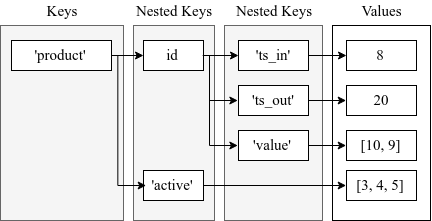
\includegraphics[width=6cm]{bab3/img/sd1.png}
	\caption{Struktur Data \textit{Dictionary} Produk}
	\label{fig:sd1}
\end{figure}

Pada struktur data produk, nilai $id$ digunakan sebagai \textit{key}.  

\begin{figure}[h]
	\centering
	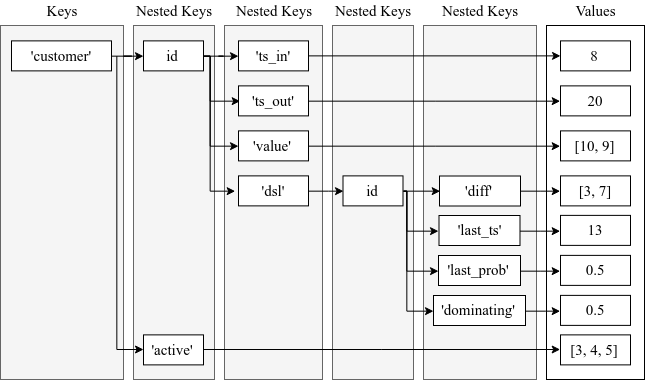
\includegraphics[width=9cm]{bab3/img/sd2.png}
	\caption{Struktur Data \textit{Dictionary} Pelanggan}
	\label{fig:sd2}
\end{figure}

 

\begin{table}[H]
	\centering
	\begin{tabular}{ | p{1.5cm} | p{7.5cm} | }
		\hline
		\textbf{Key} & \textbf{Value} \\ \hline \hline
		$id$ & ID unik data \\ \hline
		$ts\_in$ & \textit{Timestamp} masuk \\ \hline
		$ts\_out$ & \textit{Timestamp} keluar \\ \hline
		$value$ & Nilai data pada semua atribut/dimensi yang disimpan dalam bentuk \textit{array}\\ \hline
		$dsl$ & Hasil \textit{dynamic skyline} yang disimpan dalam bentuk \textit{dictionary} \\ \hline
		$diff$ & Selisih antara nilai atribut
	\end{tabular} 
	\caption{Deskripsi \textit{Key} dan \textit{Value}}
	\label{tab:desc-key}
\end{table}

\subsubsection{\textit{Event Queue}}

\subsubsection{\textit{Pandora Box}}
\tab \textit{Pandora Box} adalah sebuah struktur data array dua dimensi, sumbu $x$ adalah \textit{timestamp} dan sumbu $y$ adalah produk. Struktur data ini digunakan untuk menyimpan skor kontribusi pasar setiap waktu. Menggunakan contoh \textit{dataset} pada Tabel \ref{tab:dataset-2}, \textit{Pandora Box} yang dibutuhkan seperti di bawah ini.  



\subsection{Algoritme Utama}
\tab Sebagaimana yang telah dijelaskan sebelumnya bahwa algoritme utama terdiri dari dua tahap pemrosesan, yaitu \textit{data precomputing} dan \textit{query processing}. Secara garis besar, alur kerja sistem secara umum disajikan dalam bentuk diagram alur yang dapat dilihat pada Gambar ...

Tahap \textit{data precomputing} bertujuan untuk menghitung kontribusi pasar masing-masing produk berdasarkan preferensi pelanggan. Diawali dengan pembentukan \textit{Event Queue} untuk mencatat semua \textit{event} yang terjadi selama pemrosesan data. Kemudian, memproses \textit{event-event} tersebut menggunakan algoritme pemrosesan berdasarkan jenis \textit{event}-nya. Terakhir adalah menghitung kontribusi pasar dan menyimpannya ke dalam struktur data \textit{array} bernama \textit{Pandora Box}.

\textit{Pandora Box} kemudian digunakan sebagai \textit{input} pada tahap \textit{query processing}. Diawali dengan \textit{input} kueri pencarian berupa jumlah produk ($k$) dan interval waktu pencarian. Kemudian, mencari produk sejumlah $k$ yang memiliki total skor kontribusi pasar terbesar selama interval waktu pencarian. Terakhir adalah mengembalikan hasil kueri pencarian berupa $k$-produk yang paling menjanjikan kepada pengguna.

Untuk memudahkan interaksi antara pengguna dan sistem, dibuatlah aplikasi berbasis \textit{web} yang memudahkan pengguna meng-\textit{input}-kan data produk dan pelanggan, melihat pratinjau dan visualisasi data, meng-\textit{input}-kan kueri pencarian, serta melihat hasil kueri pencarian.   

\subsubsection{\textit{Data Precomputing}}
\tab \textit{Data precomputing} adalah sebuah proses yang dapat menunjang performa algoritme \textit{query processing} supaya dapat bekerja lebih efektif dan efisien. Tidak adanya proses \textit{data precomputing} menyebabkan pengulangan komputasi data setiap kali seseorang memasukkan kueri pencarian, sehingga komputasi data cukup dilakukan satu kali di awal (\textit{precomputing}). Berbeda halnya jika data yang digunakan adalah data \textit{streaming} yang nilainya terus berubah dalam periode waktu tertentu.
	
\newcolumntype{C}{>{\centering\arraybackslash}p{1.4em}}
\begin{table}[H]
	\caption{Contoh \textit{Dataset} \\ (a) Produk $P$ dan (b) Preferensi Pelanggan $C$ \label{tab:dataset-2}}
	\begin{subtable}{.5\linewidth}
		\small
		\centering
		\caption{}
		\begin{tabular}{|C|C|C|C|C|}
			\hline
			\multirow{2}{*}{\textbf{ID}} & \multicolumn{2}{c|}{\textbf{\textit{Timestamp}}} & \multicolumn{2}{c|}{\textbf{Nilai}} \\ \cline{2-5}
			& \textbf{$t_i$} & \textbf{$t_e$} & \textbf{$d_1$} & \textbf{$d_2$}\\ \hline \hline
			$p_1$ & 2 & 10 & 6 & 3 \\ \hline
			$p_2$ & 6 & 13 & 4 & 12 \\ \hline
			$p_3$ & 9 & 15 & 6 & 15 \\ \hline
			$p_4$ & 4 & 9 & 9 & 5 \\ \hline
			$p_5$ & 5 & 15 & 12 & 10 \\ \hline
		\end{tabular}
	\end{subtable}%
	\begin{subtable}{.5\linewidth}
		\small
		\centering
		\caption{}
		\begin{tabular}{|C|C|C|C|C|}
			\hline
			\multirow{2}{*}{\textbf{ID}} & \multicolumn{2}{c|}{\textbf{\textit{Timestamp}}} & \multicolumn{2}{c|}{\textbf{Nilai}} \\ \cline{2-5}
			 & \textbf{$t_i$} & \textbf{$t_e$} & \textbf{$d_1$} & \textbf{$d_2$}\\ \hline \hline
			$c_1$ & 1 & 8 & 2 & 8 \\ \hline
			$c_2$ & 4 & 14 & 4 & 10\\ \hline
			$c_3$ & 10 & 15 & 6 & 11\\ \hline
			$c_4$ & 3 & 8 & 8 & 12\\ \hline
			$c_5$ & 5 & 15 & 9 & 10\\ \hline
		\end{tabular}
	\end{subtable} 
\end{table}

Untuk memudahkan penjelasan algoritme, pada Tabel \ref{tab:dataset-2}, diberikan contoh \textit{dataset} produk $P$ dan preferensi pelanggan $C$ yang setiap datanya direpresentasikan sebagai titik $d$-dimensi dengan serial waktu $[t_i:t_e]$. Data dimodelkan sebagai \textit{timeline} yang diilustrasikan pada Gambar .... Setiap ada data $d \in D$ yang masuk atau keluar akan dicatat sebagai \textit{event} $e \in E$ dan dimasukkan ke dalam struktur data \textit{queue} bernama \textit{Event Queue}. Contoh \textit{Event Queue} yang terbentuk dari \textit{dataset} pada Tabel \ref{tab:dataset-2} ditunjukkan pada Tabel \ref{tab:event-queue}.

\begin{small}
	\begin{longtable}{|c|c|c|c|}
		\caption{Event Queue \label{tab:event-queue}}
		\hline
		\multicolumn{1}{|c|}{\textbf{ID \textit{Event}}} & \multicolumn{1}{c|}{\textbf{\textit{Timestamp}}} & \multicolumn{1}{c}{\textbf{ID Data}} & \multicolumn{1}{|c|}{\textbf{Aksi}} \\ \hline 
		\endfirsthead
		\hline
		\multicolumn{1}{|c|}{\textbf{ID \textit{Event}}} & \multicolumn{1}{c|}{\textbf{\textit{Timestamp}}} & \multicolumn{1}{c}{\textbf{ID Data}} & \multicolumn{1}{|c|}{\textbf{Aksi}} \\ \hline
		\endhead
		$e_1$ & 1 & $c_1$ & Masuk \\ \hline
		$e_2$ & 2 & $p_1$ & Masuk \\ \hline
		$e_3$ & 3 & $c_4$ & Masuk \\ \hline
		$e_4$ & 4 & $p_4$ & Masuk \\ \hline
		$e_5$ & 4 & $c_2$ & Masuk \\ \hline
		$e_6$ & 5 & $p_5$ & Masuk \\ \hline
		$e_7$ & 5 & $c_5$ & Masuk \\ \hline
		$e_8$ & 6 & $p_2$ & Masuk \\ \hline
		$e_9$ & 8 & $c_1$ & Keluar \\ \hline
		$e_{10}$ & 8 & $c_4$ & Keluar \\ \hline
		$e_{11}$ & 9 & $p_3$ & Masuk \\ \hline
		$e_{12}$ & 9 & $p_4$ & Keluar \\ \hline
		$e_{13}$ & 10 & $c_3$ & Masuk \\ \hline
		$e_{14}$ & 10 & $p_1$ & Keluar \\ \hline
		$e_{15}$ & 13 & $p_2$ & Keluar \\ \hline
		$e_{16}$ & 14 & $c_2$ & Keluar \\ \hline
		$e_{17}$ & 15 & $p_3$ & Keluar \\ \hline
		$e_{18}$ & 15 & $p_5$ & Keluar \\ \hline
		$e_{19}$ & 15 & $c_3$ & Keluar \\ \hline
		$e_{20}$ & 15 & $c_5$ & Keluar \\ \hline
	\end{longtable}
\end{small}

Kemudian, \textit{event-event} ini akan diproses secara berurutan menggunakan algoritme yang sesuai dengan jenis \textit{event}-nya. Ada empat jenis proses yang dilakukan berdasarkan jenis \textit{event}, yaitu: (1) produk masuk (\textit{product insertion}), (2) produk keluar (\textit{product deletion}), (3) pelanggan masuk (\textit{customer insertion}), dan (4) pelanggan keluar (\textit{customer deletion}). 

Terlepas dari empat jenis pemrosesan \textit{event}, sebenarnya hanya ada dua jenis komputasi \textit{skyline} yang digunakan dalam \textit{data precomputing}, yaitu \textit{dynamic skyline} dan \textit{reverse skyline}. Dua komputasi tersebut digunakan sebagai metode perhitungan probabilitas dan kontribusi pasar. 

\myparagraph{Komputasi \textit{Dynamic Skyline}}

Sebagaimana yang telah dijelaskan pada Bab Tinjauan Pustaka, komputasi \textit{dynamic skyline} digunakan untuk mencari produk terbaik dari sudut pandang pelanggan \cite{kmpp}. \textit{Dynamic skyline} \cite{dynamic-skyline} dari seorang pelanggan $c_1 \in C$, dinotasikan dengan $DSL(c_1)$, berisi semua produk $p_1 \in P$ yang tidak didominasi oleh produk lain $p_2 \in P$ berdasarkan preferensi pelanggan $c_1$, $p_2 \nprec_{c_1} p_1$. 

Proses komputasi \textit{dynamic skyline} diawali dengan perhitungan selisih absolut dari nilai masing-masing dimensi antara pelanggan dan produk, dinotasikan dengan:
\begin{equation}\label{eq:diff}
diff^i = |c_1^i - p^i|
\end{equation}

Selanjutnya, mengecek dominansi dinamis antar produk dengan membandingkan selisih absolut-nya. Misalnya, ada dua produk yang akan dibandingkan, dinotasikan dengan $p_s$ sebagai subjek yang dibandingkan dan $p_o$ sebagai objek pembanding. Berdasarkan syarat dominansi dinamis (Persamaan \ref{eq:syarat-dominansi-dinamis}), $p_s$ dikatakan mendominasi $p_o$ jika dan hanya jika:
\begin{equation}\label{eq:komputasi-dsl}
\begin{split}
\text{(a)} \tab diff_s^i \leq diff_o^i, \forall i \in [1, ..., d] \\
\text{(b)} \tab diff_s^i < diff_o^i, \exists i \in [1, ..., d]
\end{split}
\end{equation}

Pengecekan dominansi dinamis ini dilakukan secara iteratif sampai dipastikan suatu $p_1$ tidak didominasi oleh $p_2$ lain sama sekali. Jika $p_1$ pernah didominasi, maka $p_1$ tidak dapat menjadi hasil \textit{dynamic skyline}.

Menggunakan contoh \textit{dataset} pada Tabel \ref{tab:dataset-2}, dengan mengabaikan \textit{timestamp}-nya akan didapatkan perhitungan hasil \textit{dynamic skyline} seperti pada Tabel \ref{tab:dsl-res}.

\begin{table}[H]
	\small
	\centering
	\begin{tabular}{|p{2cm}|p{3cm}|}
		\hline
		$DSL(c_1)$ & $\{2, 4, 5\}$ \\ \hline
		$DSL(c_2)$ & $\{2, 5\}$ \\ \hline
		$DSL(c_3)$ & $\{2, 3\}$ \\ \hline
		$DSL(c_4)$ & $\{2, 3, 4\}$\\ \hline
		$DSL(c_5)$ & $\{4, 5\}$ \\ \hline
	\end{tabular} 
	\caption{Hasil Perhitungan \textit{Dynamic Skyline} dari \textit{Dataset} \ref{tab:dataset-2}}
	\label{tab:dsl-res}
\end{table}


\myparagraph{Komputasi \textit{Reverse Skyline}}

Komputasi \textit{reverse skyline} digunakan untuk mencari pelanggan potensial dari sudut pandang produsen \cite{kmpp}. \textit{Reverse skyline} \cite{reverse-skyline} dari sebuah produk $p_1 \in
P$, dinotasikan dengan $RSL(p_1)$, berisi semua pelanggan $c \in C$ yang memiliki $p_1$ pada hasil \textit{dynamic skyline}-nya.

Sebagaimana yang telah dijelaskan pada Tinjauan Pustaka, komputasi \textit{reverse skyline} diawali dengan menentukan \textit{orthant} dari produk, dinotasikan dengan $O$. Dalam geometri, \textit{orthant} adalah analog dalam ruang data \textit{d}-dimensi atau biasa dikenal sebagai kuadran dalam bidang dua dimensi. Setiap produk $p$ memiliki $2^d$ \textit{orthant} pada data $d-$dimensi. 

\textit{Orthant} ditandai menggunakan bilangan biner. Sebagai contoh, terdapat empat \textit{orthant} pada bidang dua dimensi, yaitu $O_{00}$, $O_{01}$, $O_{10}$, dan $O_{11}$, dan delapan \textit{orthant} pada bidang tiga dimensi, yaitu $O_{000}$, $O_{001}$, $O_{010}$, $O_{011}$, $O_{100}$, $O_{101}$, $O_{110}$ dan $O_{111}$. Penggunaan bilangan biner bertujuan untuk menandai batas wilayah sebuah \textit{orthant}. Misalnya, \textit{orthant} $O_{010}$ dari produk $p_1$ memiliki wilayah dengan batas-batas sebagai berikut: sumbu $x$ (0 - $pos_x(p_1)$), sumbu $y$ ($pos_y(p_1)$ - $max_y$), dan sumbu $z$ (0 - $pos_z(p_1)$).

Langkah selanjutnya adalah menghitung \textit{midpoint} atau titik tengah antara produk kueri dan produk lainnya, misalnya $p_1$ (sebagai titik kueri) dan $p_2 \in P$, menggunakan rumus berikut: 
\begin{equation} \label{eq:midpoint2}
m_2^i = \frac{(p_1^i + p_2^i)}{2}
\end{equation}
Kemudian, menentukan \textit{midpoint skyline} atau \textit{mid-skyline} \cite{mid-skyline} pada setiap \textit{orthant}.

Langkah terakhir adalah mengecek setiap pelanggan $c \in C$ apakah didominasi oleh hasil \textit{mid-skyline} pada masing-masing \textit{orthant} atau tidak (Persamaan \ref{eq:mid-skyline}). Jika $c$ didominasi, maka $c$ tidak dapat menjadi hasil \textit{reverse skyline}.

\myparagraph{Perhitungan Probabilitas}

Setelah mendapatkan hasil \textit{dynamic skyline} pada Tabel \ref{tab:dsl-res}, selanjutnya adalah menghitung probabilitas masing-masing produk $p$ dipilih oleh pelanggan $c$, dinotasikan dengan $Pr(c, p|P)$, yang telah dijelaskan pada Persamaan \ref{eq:probability}. Sehingga, dari Tabel \ref{tab:dsl-res} akan didapatkan hasil perhitungan probabilitas sebagai berikut.

\begin{small}
	\begin{longtable}{|p{1.5cm}|p{3cm}|p{2.5cm}|}
		\caption{Hasil Perhitungan Probabilitas dari Tabel \ref{tab:dsl-res}}
		\label{tab:prob-res}
		\hline
		\multirow{5}{*}{$p_1$} & $Pr(c_1, p_1|P)$ & $0$ \\ \cline{2-3}
		& $Pr(c_2, p_1|P)$ & $0$ \\ \cline{2-3}
		& $Pr(c_3, p_1|P)$ & $0$ \\ \cline{2-3}
		& $Pr(c_4, p_1|P)$ & $0$ \\ \cline{2-3}
		& $Pr(c_5, p_1|P)$ & $0$ \\ \hline
		\multirow{5}{*}{$p_2$} & $Pr(c_1, p_2|P)$ & $\frac{1}{3} = 0.33$ \\ \cline{2-3}
		& $Pr(c_2, p_2|P)$ & $\frac{1}{2} = 0.5$ \\ \cline{2-3}
		& $Pr(c_3, p_2|P)$ & $\frac{1}{2} = 0.5$ \\ \cline{2-3}
		& $Pr(c_4, p_2|P)$ & $\frac{1}{3} = 0.33$  \\ \cline{2-3}
		& $Pr(c_5, p_2|P)$ & $0$ \\ \hline
		\multirow{5}{*}{$p_3$} & $Pr(c_1, p_3|P)$ & $0$ \\ \cline{2-3}
		& $Pr(c_2, p_3|P)$ & $0$ \\ \cline{2-3}
		& $Pr(c_3, p_3|P)$ & $\frac{1}{2} = 0.5$ \\ \cline{2-3}
		& $Pr(c_4, p_3|P)$ & $\frac{1}{3} = 0.33$  \\ \cline{2-3}
		& $Pr(c_5, p_3|P)$ & $0$ \\ \hline
		\multirow{5}{*}{$p_4$} & $Pr(c_1, p_4|P)$ & $\frac{1}{3} = 0.33$ \\ \cline{2-3}
		& $Pr(c_2, p_4|P)$ & $0$ \\ \cline{2-3}
		& $Pr(c_3, p_4|P)$ & $0$ \\ \cline{2-3}
		& $Pr(c_4, p_4|P)$ & $\frac{1}{3} = 0.33$  \\ \cline{2-3}
		& $Pr(c_5, p_4|P)$ & $\frac{1}{2} = 0.5$ \\ \hline
		\multirow{5}{*}{$p_5$} & $Pr(c_1, p_5|P)$ & $\frac{1}{3} = 0.33$ \\ \cline{2-3}
		& $Pr(c_2, p_5|P)$ & $\frac{1}{2} = 0.5$ \\ \cline{2-3}
		& $Pr(c_3, p_5|P)$ & $0$ \\ \cline{2-3}
		& $Pr(c_4, p_5|P)$ & $0$  \\ \cline{2-3}
		& $Pr(c_5, p_5|P)$ & $\frac{1}{2} = 0.5$ \\ \hline
	\end{longtable}
\end{small}

\myparagraph{Perhitungan Kontribusi Pasar (\textit{Market Contribution})}

Hasil perhitungan probabilitas produk $p$ pada Tabel \ref{tab:prob-res} kemudian diakumulasikan menjadi skor kontribusi pasar sebagaimana yang dijelaskan pada Persamaan \ref{eq:market-contr}. Sehingga akan didapatkan hasil pada Tabel \ref{tab:mc-res}.

\begin{table}[H]
	\small
	\centering
	\begin{tabular}{|p{3cm}|p{2cm}|}
		\hline
		$E(C, p_1|P)$ & $0$ \\ \hline
		$E(C, p_2|P)$ & $1.66$ \\ \hline
		$E(C, p_3|P)$ & $0.83$ \\ \hline
		$E(C, p_4|P)$ & $1.16$ \\ \hline
		$E(C, p_5|P)$ & $1.33$ \\ \hline
	\end{tabular} 
	\caption{Hasil Perhitungan Kontribusi Pasar dari Tabel \ref{tab:prob-res}}
	\label{tab:mc-res}
\end{table}

\myparagraph{Proses \textit{Product Insertion}}

Proses \textit{Product Insertion} adalah proses yang dijalankan ketika ada produk yang masuk ke dalam \textit{timeline}. Ketika ada data produk yang masuk, ada kemungkinan jika produk tersebut menjadi hasil \textit{dynamic skyline} suatu pelanggan $c \in C$ sehingga mengubah hasil perhitungan probabilitasnya. Hasil dari proses ini adalah \textit{Pandora Box} yang telah diperbarui.

Algoritme pemrosesan yang dilakukan adalah:
\begin{enumerate}
	\item Menambah produk $p$ ke dalam daftar produk aktif, dinotasikan dengan $P_a$
	\item Menghitung $RSL(p)$
	\item Menghitung $DSL(c), \forall c \in RSL(p)$ 
	\item Memperbarui \textit{Pandora Box}
\end{enumerate}

\myparagraph{Proses \textit{Product Deletion}}

Proses \textit{Product Deletion} adalah proses yang dijalankan ketika ada produk yang keluar dari \textit{timeline}. Produk yang keluar dinotasikan dengan $p_{out}$. Ketika ada data produk yang keluar, ada kemungkinan jika produk tersebut menjadi hasil \textit{dynamic skyline} suatu pelanggan $c \in C$ sehingga mengubah hasil perhitungan probabilitasnya. Sama seperti proses \textit{product insertion}, hasil dari proses ini adalah \textit{Pandora Box} yang telah diperbarui.

Algoritme pemrosesan yang dilakukan adalah:
\begin{enumerate}
	\item Memperbarui \textit{Pandora Box}
	\item Menghitung $RSL(p_{out})$
	\item Menghitung $DSL(c), \forall c \in RSL(p_{out})$
	\item Menghapus produk $p$ ke dalam daftar produk aktif, dinotasikan dengan $P_a$
\end{enumerate}

\myparagraph{Proses \textit{Customer Insertion}}

Proses \textit{Customer Insertion} adalah proses yang dijalankan ketika ada pelanggan yang masuk ke dalam \textit{timeline}. 

Algoritme pemrosesan yang dilakukan adalah:
\begin{enumerate}
	\item Menambah pelanggan $c$ ke dalam daftar pelanggan aktif, dinotasikan dengan $C_a$
	\item Menghitung \textit{Initial} $DSL(c)$ 
	\item Memperbarui \textit{Pandora Box}
\end{enumerate}

\myparagraph{Proses \textit{Customer Deletion}}

Proses \textit{Customer Deletion} adalah proses yang dijalankan ketika ada pelanggan yang keluar dari \textit{timeline}. 

Algoritme pemrosesan yang dilakukan adalah:
\begin{enumerate}
	\item Memperbarui \textit{Pandora Box}
	\item Menghapus pelanggan $c$ dari daftar pelanggan aktif $C_a$
\end{enumerate}

\subsubsection{\textit{Query Processing}}

\subsection{Algoritme \textit{Brute Force}}

\subsection{Arsitektur Aplikasi} 
\tab Sistem akan diimplementasikan menggunakan arsitektur \textit{client}-\textit{server} dan antarmuka pengguna grafis berbasis situs web, sebagaimana yang diilustrasikan pada Gambar ... Terdapat dua komponen utama dalam arsitektur ini, yakni:

\begin{enumerate}
	\item Client
	
	\tab Menampilkan antarmuka pengguna grafis berbasis situs web. 
\end{enumerate}